\documentclass[a4paper,14pt]{extreport}
\usepackage[left=1.5cm,right=1.5cm,
    top=1.5cm,bottom=2cm,bindingoffset=0cm]{geometry}
\usepackage{scrextend}
\usepackage[T1,T2A]{fontenc}
\usepackage[utf8]{inputenc}
\usepackage[english,russian,ukrainian]{babel}
\usepackage{tabularx}
\usepackage{amssymb}
\usepackage{color}
\usepackage{amsmath}
\usepackage{mathrsfs}
\usepackage{listings}
\usepackage{graphicx}
\graphicspath{ {./images/} }
\usepackage{lipsum}
\usepackage{xcolor}
\usepackage{hyperref}

\usepackage{tcolorbox}
\usepackage{tikz}
\usepackage[framemethod=TikZ]{mdframed}
\usepackage{wrapfig,boxedminipage,lipsum}
\mdfdefinestyle{MyFrame}{%
linecolor=blue,outerlinewidth=2pt,roundcorner=20pt,innertopmargin=\baselineskip,innerbottommargin=\baselineskip,innerrightmargin=20pt,innerleftmargin=20pt,backgroundcolor=gray!50!white}
 \usepackage{csvsimple}
 \usepackage{supertabular}
\usepackage{pdflscape}
\usepackage{fancyvrb}
%\usepackage{comment}
\definecolor{ggreen}{rgb}{0.,1,0}
\definecolor{rred}{rgb}{1,0.1,0.1}
\usepackage{array,tabularx}
\usepackage{colortbl}

\usepackage{varwidth}
\tcbuselibrary{skins}
\usepackage{fancybox}




\usepackage{float}
\usepackage{wrapfig}
\usepackage{framed}





\begin{document}

\tableofcontents

\chapter{Хвилі в хвилеводах}
\section{1. Вид закону дисперсії хвиль у хвилеводах. Які його асимптоти?}
\begin{center}

$\upsilon_{\text{ф}} = \dfrac{c}{\sqrt{(\dfrac{\lambda_{\text{кр}}}{\lambda})^2}}$\\

Cпiввiдношення показує, що фазова швидкiсть
залежить вiд частоти, i характеризує закон дисперсiї для хвилеводу
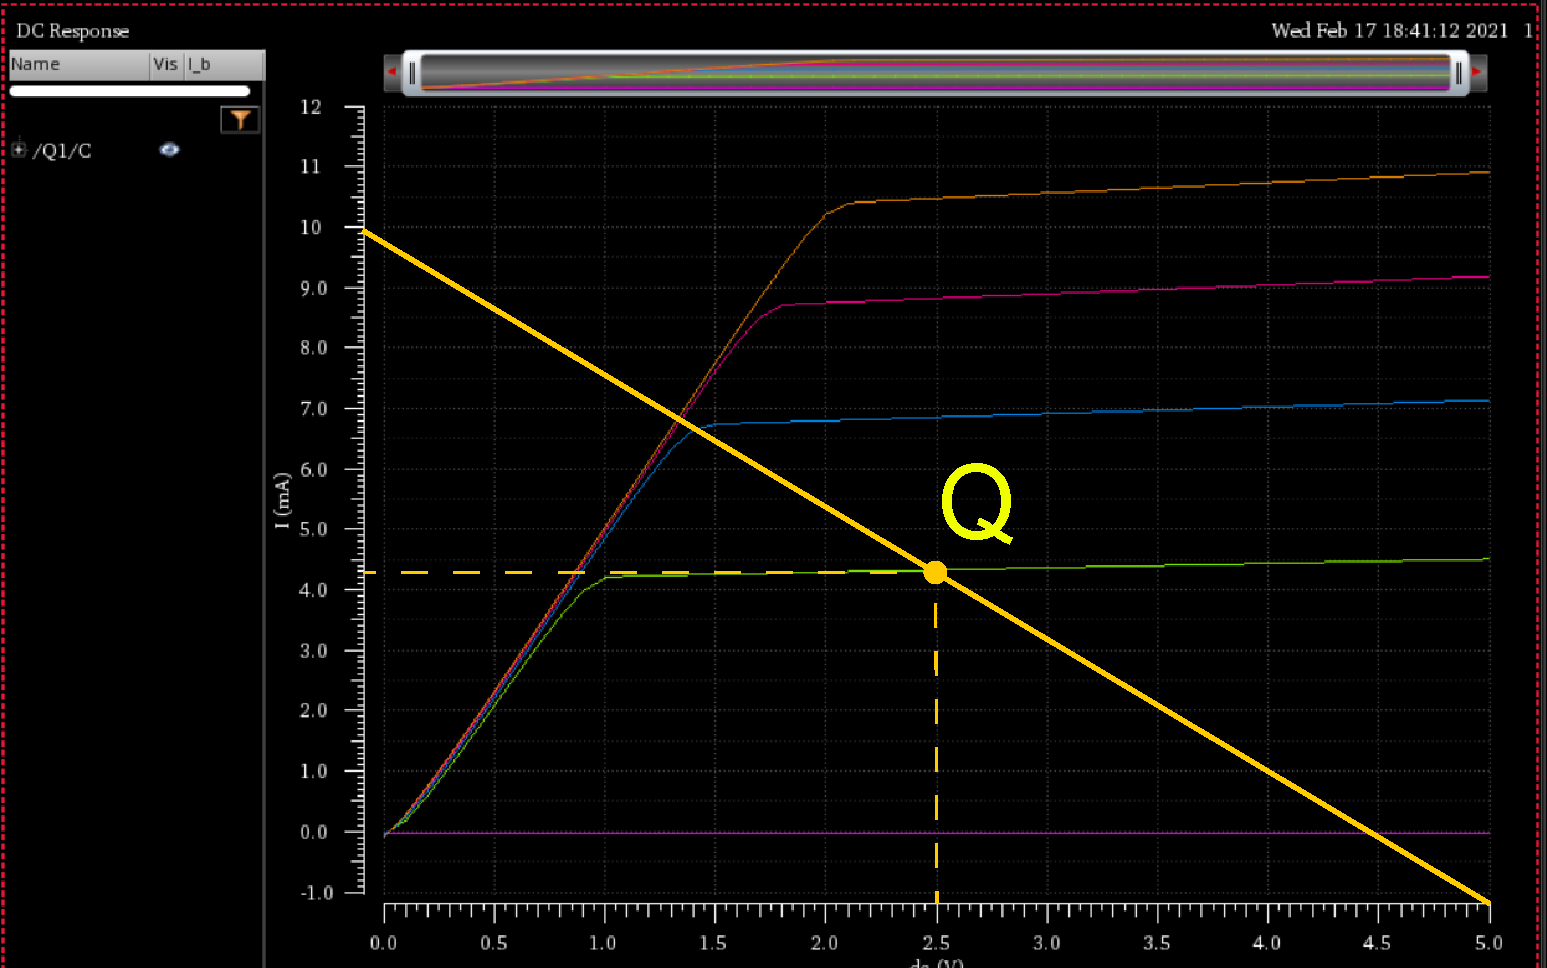
\includegraphics[scale=0.7]{1.png}
\end{center}\par
Oсобливiсть даного закону пов'язана з тим, що
дiйснi значення фазової швидкостi, а значить, i
нормальне розповсюдження електромагнiтних хвиль по
хвилеводу можливе лише для областi частот f > fкр. Звiдси зрозумiлим стає фiзичний змiст позначення fкр: критична частота – це гранична частота, що подiляє дiапазон нормального розповсюдження електромагнiтних полiв у виглядi хвиль i так званий дiапазон вiдсiчки f < fкр.\par
Закон дисперсії визначає ще одну корисну залежність –
групової швидкості від частоти: добуток групової і фазової
швидкості дорівнює квадрату швидкості світла $\upsilon_{\text{ф}}\upsilon_{\text{гр}} = c^2$.\par
\textbf{Oсобливості поведiнки електромагнiтних полiв у режимi
вiдсiчки.} Якщо будемо намагатися збуджувати хвилевід на частотi,
нижчiй за критичну, то фазова швидкiсть,
довжина хвилi, а значить, i хвильове число у хвилеводi повиннi бути
уявними величинами. Тому хвильовi множники в (5.2) приймають
форму $e^{\pm|K|z} e^{i\omega t}$
, яка показує, що складовi поля у всiх точках
хвилеводу коливаються синфазно у часi, а амплiтуда коливань
вздовж хвилеводу спадає експоненцiально.


\section{2. Що таке fкр, від чого вона залежить? Які умови поширення?}
Критична частота – це гранична частота, що подiляє
дiапазон нормального розповсюдження електромагнiтних
полiв у виглядi хвиль i так званий дiапазон вiдсiчки f < fкр.

\section{3. Що таке позамежний хвилевід? Що в ньому відбувається?}
Такой, в котором волна может распространяться на частоте, меньшей за критическую. Волна распространяется в режиме отсечки (fкр = 0). Параметры волны становятся мнимыми величинами

\section{4. Типи хвиль у хвилеводах.}
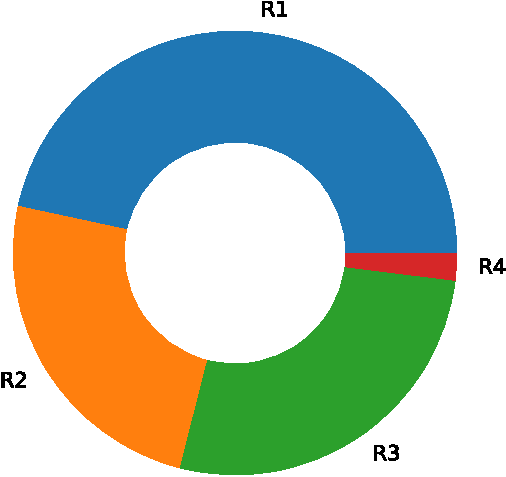
\includegraphics[scale=0.58]{2.png}\par
TEMхвиля (Ez = Hz = 0), необхiдною умовою існування є рiвнiсть K = k.
Для таких хвиль характерна вiдсутнiсть дисперсiї ($\upsilon_{\text{ф}}$ = c).\\
K -- поздовжнє хвильове число\\
к -- хвильове число\\

\section{5. Які особливості ТЕМ-хвилі? У яких хвилеводах вона може поширюватися?}
TEMхвиля (Ez = Hz = 0), необхiдною умовою існування є рiвнiсть K = k.
Для таких хвиль характерна вiдсутнiсть дисперсiї ($\upsilon_{\text{ф}}$ = c).\\
K -- поздовжнє хвильове число\\
к -- хвильове число\\
Хвилi TEM, розподiл
поперечних полiв для яких такий саме, як i статичних, за заданої
конфiгурацiї хвилеводу мають єдиний розв'язок рiвнянь Лапласа i,
отже, не мають рiзновидностей.\\

Основним типом хвилi для \textbf{коаксiального хвилеводу} є TEMхвиля, яка характеризується вiдсутнiстю дисперсiї i як наслiдок -
рiвнiстю фазової швидкостi й швидкостi свiтла для данного
дiелектричного середовища. Характер розподiлу полiв у поперечній
площині для TEM-хвиль, що бiжать, спiвпадає з розподiлом
статичних полiв i знаходиться з рiвняння Лапласа.\\

Смужкові лінії передачі та Мікросмужкові лінії Цей тип ліній передачі використовується в основному для
поширення ТЕМ-хвиль, для яких фазова швидкість дорівнює
швидкості світла у вільному просторі з урахуванням діелектричного
заповнення. Проте підвищення частоти вносить зміни у структуру
поля, створюючи так звану квазі-ТЕМ хвилю. Префікс «квазі»
вказує на наявність поздовжніх складових полів, зростання яких з
підвищенням частоти призводить до прояву дисперсії. Причина їх
появи описана в розд. 2.3.3 і викликана скінченим опором смужки,
який зростає за рахунок скін-ефекту. Інший фактор пов'язаний з
перерозподілом енергії між діелектричним та повітряним
середовищем і відповідною зміною ефективної діелектричної
проникності.


\section{6. Структура полів основної моди в прямокутному хвилеводі.}
хвилі з різноманітними конфігураціями
полів їх називають, модами.\\
Одномодовий режим, тобто на тих частотах, на яких у хвилеводi
може розповсюджуватись лише одна мода.\\
Електричнi силовi лiнiї мають лише
одну складову i з'єднують широкi стiнки. Найбiльше значення Ey
має у центрi хвилеводу, а на бiчних стiнках зменшується до нуля.
Магнiтнi силовi лiнiї являють собою замкненi лiнiї, що лежать в
площинах, паралельних широким стiнкам. ???????????????????????

\section{7. Структура полів основної моди в коаксіальному хвилеводі.}
Коаксiальний хвилевід – найбiльш розповсюджена
лiнiя передачi. Використовуються як твердi, наповненi
повiтрям хвилеводи (фідери), так i гнучкi, з дiелектричним
заповненням (коаксiальнi кабелi).
НЕЕБУ Характер розподiлу полiв у поперечній
площині для TEM-хвиль, що бiжать, спiвпадає з розподiлом
статичних полiв i знаходиться з рiвняння Лапласа.


\section{8. Діелектричні хвилеводи, їхні структури й області застосування.}
Альтернативною передавальною лінією у зазначеному
діапазоні більш коротких (міліметрових, субміліметрових) довжин хвиль є діелектричний хвилевід. На відміну від металевих, в основу принципу дії в діелектричних хвилеводах. покладено явище повного внутрішнього
відбивання електромагнітної хвилі, яке спостерігається на межі
поділу двох діелектриків (див. розд. 4.3.3.).
Характерною особливістю
повного внутрішнього відбивання є існування так званої поверхневої
хвилі по той бік поверхні відбивання, яка створюється крайовими
полями, котрі «провисають» через межу поділу. Амплітуда цієї
хвилі спадає з віддаленням від межі, і тим сильніше, чим кут
падіння більший за граничне значення (4.40).\\
\textbf{Круглий діелектричний хвилевід}\\
\textbf{Плоский діелектричний хвилевід}\\
\textbf{Оптоволокно}\\



\section{9. Смужкові хвилеводи, їхні структури й області застосування.}
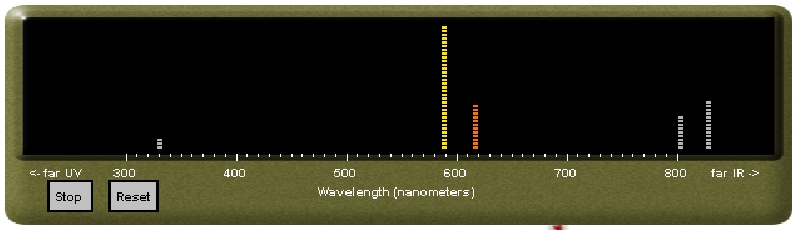
\includegraphics[scale=1]{3.png}\par
\textbf{Мікросмужкові ліні}\\
Розрізняють два типи мікросмужкових ліній: симетричні і
несиметричні. Симетрична СЛП конструктивно
складається з двох металевих площин, що розділені діелектриком зі
вставкою металевої смужки.\\
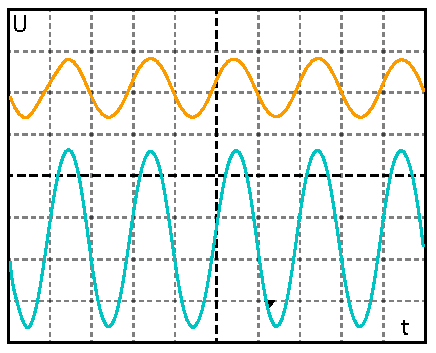
\includegraphics[scale=0.6]{4.png}\par

\textbf{Щілинна лінія}\\
\textbf{Копланарна лінія}\\
У даний час запропоновано велику кількість типів напрямних
ліній (у тому числі і смужкові), які крім виконання основного
призначення, є гнучким інструментом конструювання елементів,
функціональних вузлів, блоків НВЧ різного призначення. Смужкові
напрямні системи застосовують у діапазоні 0,1 - 30 ГГц і навіть у
міліметровому діапазоні довжин хвиль.


\section{10. Способи збудження хвиль у хвилеводах.}
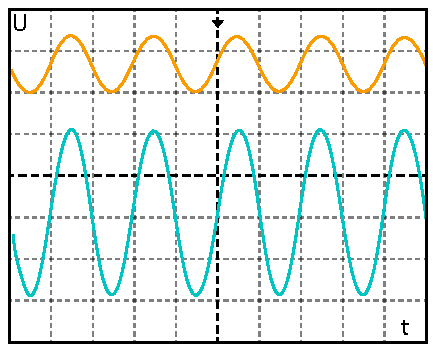
\includegraphics[scale=0.9]{9.png}\par
\section{11. На чому заснована можливість схемного представлення хвилеводних елементів? Які необхідні умови потрібні для цього?}

\chapter{Резонатори}
\section{1. Що таке резонатор для НВЧ діапазону, які його особливості, чим він відрізняється від коливального контуру}
Резонатор є коливальною системою, в якій можливе
існування власних коливань на певних частотах, званих
резонансними. Резонансні властивості мають різні коливальні
системи: натягнута струна, маятник, коливальний контур,
пружна пластина, пружина і так далі. Резонансна частота
коливальної системи залежить від її параметрів. Так для
маятника - важка на нитці - частота власних коливань
визначається масою важка і довжини нитки, а у разі
коливального контура - номіналами його реактивних
компонентів(ємності і індуктивності).
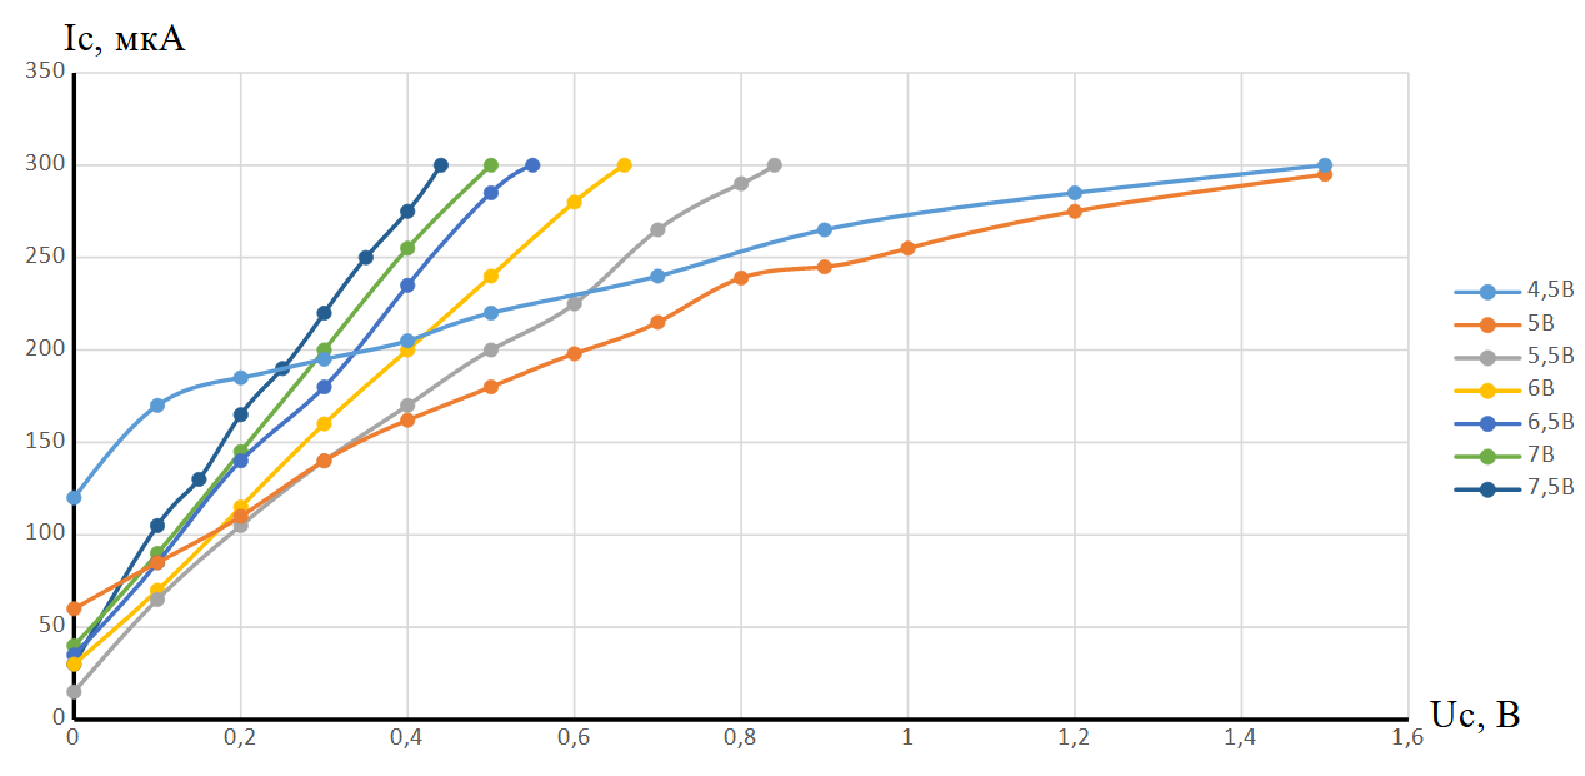
\includegraphics[scale=0.9]{5.png}\par
З метою просування в область НВЧ-діапазону - необхідно зменшувати
ємність конденсатора і величину індуктивності котушки. Слід зазначити, що коливальний контур використовується на низьких
частотах, за яких геометричні розміри коливальної системи істотно
менші за довжину хвилі. Це пов'язано з тим, що, по-перше,
виготовлення реактивних елементів, що характеризуються
мінімальними значеннями зосереджених параметрів, зв'язане з
рядом труднощів. По-друге, у НВЧ діапазоні геометричні розміри
вказаної системи стають порівнянними з довжиною хвилі, що
призводить до випромінювання накопичуваної енергії у навколишній
простір і, значить, до втрати резонансних властивостей.
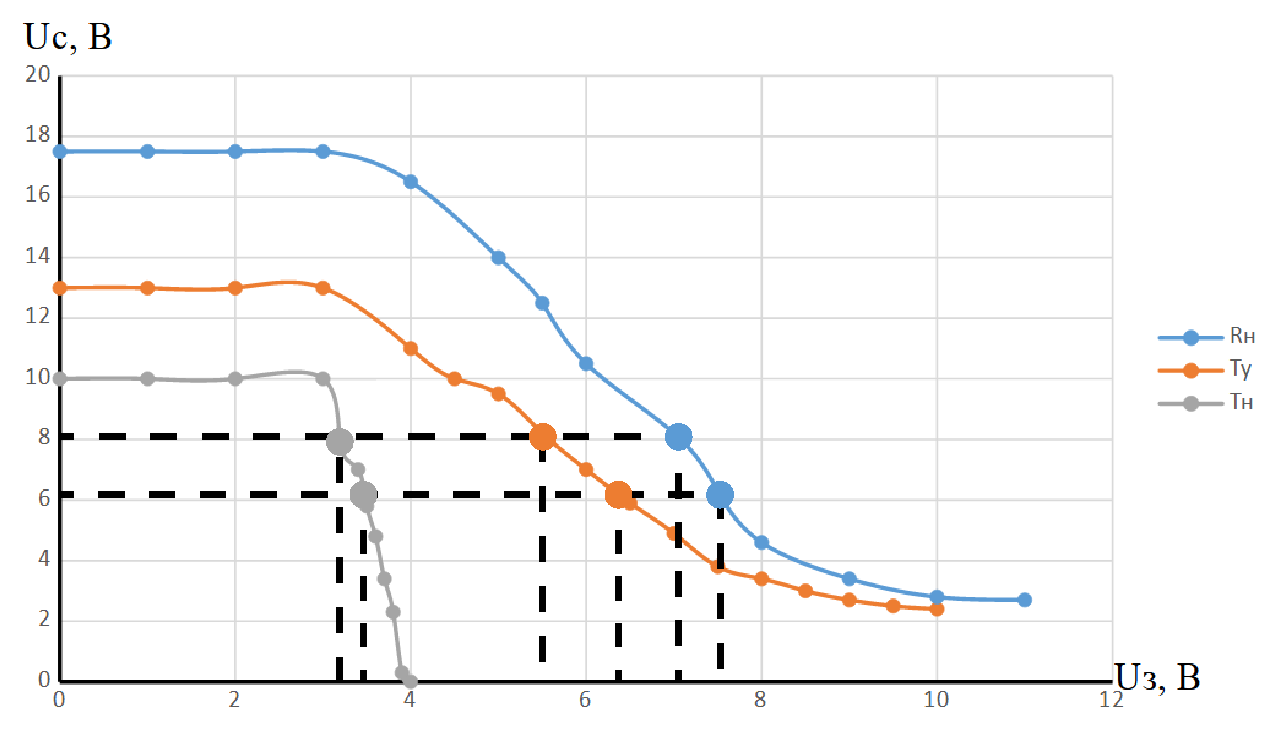
\includegraphics[scale=0.9]{6.png}\par
\section{2. Від чого залежить власна частота резонатора?}
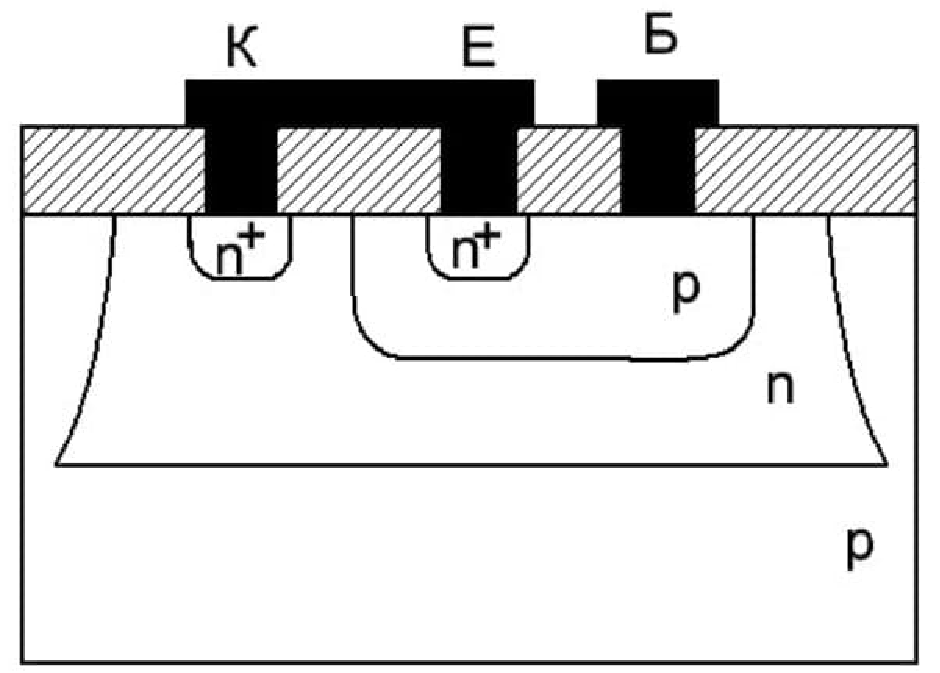
\includegraphics[scale=0.9]{7.png}\par
\section{3. Чим відрізняється півхвильовий резонатор від чвертьхвильового, які умови резонансу?}
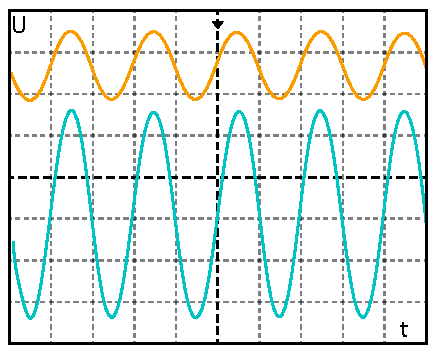
\includegraphics[scale=0.9]{8.jpg}\par





\end{document}
